\documentclass[paper=letter, fontsize=11pt]{scrartcl} 

\usepackage{graphicx}
\usepackage{verbatim}
\usepackage{pictex}  
\usepackage{multimedia}
\usepackage{listings}
\usepackage{xcolor,colortbl}
\usepackage[spanish]{babel} % language/hyphenation
\usepackage[utf8]{inputenc}
\usepackage{amsmath,amsfonts,amsthm} % Math packages
\usepackage{amsbsy}
\usepackage{amssymb}
\usepackage{fancyvrb}
\usepackage{sectsty} % Allows customizing section commands
\allsectionsfont{\centering \normalfont\scshape} % Make all sections centered, the default font and small caps

\usepackage{fancyhdr} % Custom headers and footers
\pagestyle{fancyplain} % Makes all pages in the document conform to the custom headers and footers
\fancyhead{} % No page header - if you want one, create it in the same way as the footers below
\fancyfoot[L]{} % Empty left footer
\fancyfoot[C]{} % Empty center footer
\fancyfoot[R]{\thepage} % Page numbering for right footer
\renewcommand{\headrulewidth}{0pt} % Remove header underlines
\renewcommand{\footrulewidth}{0pt} % Remove footer underlines
\setlength{\headheight}{13.6pt} % Customize the height of the header

\numberwithin{equation}{section} % Number equations within sections (i.e. 1.1, 1.2, 2.1, 2.2 instead of 1, 2, 3, 4)
\numberwithin{figure}{section} % Number figures within sections (i.e. 1.1, 1.2, 2.1, 2.2 instead of 1, 2, 3, 4)
\numberwithin{table}{section} % Number tables within sections (i.e. 1.1, 1.2, 2.1, 2.2 instead of 1, 2, 3, 4)

\setlength\parindent{0pt} % Removes all indentation from paragraphs - comment this line for an assignment with lots of text
\lstset{language=R,literate={<-}{{$\gets$}}1}
\newcommand{\horrule}[1]{\rule{\linewidth}{#1}} % Create horizontal rule command with 1 argument of height

\title{	
\normalfont \normalsize 
\textsc{Centro de Investigaci\'on en Matem\'aticas (CIMAT). Unidad Monterrey} 
\\ [25pt] 
\horrule{0.5pt} \\[0.4cm] % Thin top horizontal rule
\huge Matrices aleatorias: Tarea 1\\ 
\horrule{2pt} \\[0.5cm] % Thick bottom horizontal rule
}

\author{Jorge Luis Ramos Zavaleta} % Your name

\date{\normalsize\today} % Today's date or a custom date

\begin{document}
\lstdefinestyle{customc}{
  belowcaptionskip=1\baselineskip,
  basicstyle=\footnotesize, 
  frame=lrtb,
  breaklines=true,
  %frame=L,
  %xleftmargin=\parindent,
  language=C,
  showstringspaces=false,
  basicstyle=\footnotesize\ttfamily,
  keywordstyle=\bfseries\color{green!40!black},
  commentstyle=\itshape\color{red!40!black},
  identifierstyle=\color{blue},
  stringstyle=\color{purple},
}

\lstset{breakatwhitespace=true,
  basicstyle=\footnotesize, 
  commentstyle=\color{green},
  keywordstyle=\color{blue},
  stringstyle=\color{purple},
  language=C++,
  columns=fullflexible,
  keepspaces=true,
  breaklines=true,
  tabsize=3, 
  showstringspaces=false,
  extendedchars=true}

\lstset{ %
  language=R,    
  basicstyle=\footnotesize, 
  numbers=left,             
  numberstyle=\tiny\color{gray}, 
  stepnumber=1,              
  numbersep=5pt,             
  backgroundcolor=\color{white},
  showspaces=false,             
  showstringspaces=false,       
  showtabs=false,               
  frame=single,                 
  rulecolor=\color{black},      
  tabsize=2,                  
  captionpos=b,               
  breaklines=true,            
  breakatwhitespace=false,    
  title=\lstname,             
  keywordstyle=\color{blue},  
  commentstyle=\color{dkgreen},
  stringstyle=\color{mauve},   
  escapeinside={\%*}{*)},      
  morekeywords={*,...}         
} 


\maketitle % Print the title


\section{Ejercicio}

De las diapositivas correspondientes a esta sesión, completar los
pasos para llegar de la ec. 6 a la ec. 9.


\subsection{Soluci\'on}
Tenemos que $$f(x,t+\tau)=\int_{-\infty}^{\infty}d\Delta \rho(\Delta)f(x-\Delta,t)$$ Expandiendo el lado izquierdo en su serie de Taylor alrededor de $\tau$ tenemos que $$f(x,t+\tau)=f(x,t)+\tau \frac{df}{dt}+...$$ Ahora expandiendo $f(x-\Delta, t)$ alrededor de $\Delta$ $$f(x-\Delta, t)=f(x,t)-\Delta \frac{df}{dx}+\frac{\Delta^2}{2}\frac{d^2 f}{dx^2}+...$$ Sustituyendo tenemos que \begin{equation*}
\begin{split}
f(x,t)+\tau \frac{df}{dt}+...&=\int_{-\infty}^{\infty}d\Delta\rho(\Delta)\left[f(x,t)-\Delta \frac{df}{dx}+\frac{\Delta^2}{2}\frac{d^2 f}{dx^2}+...\right]\\
&= f(x,t)\int_{-\infty}^{\infty}d\Delta\rho(\Delta)-\frac{df}{dx}\int_{-\infty}^{\infty}\Delta d\Delta\rho(\Delta)+\frac{1}{2}\frac{d^2 f}{dx^2}\int_{-\infty}^{\infty}\Delta^2 d\Delta\rho(\Delta) +...
\end{split}
\end{equation*}
Ahora por la propiedad de normalizaci\'on, es decir, dado que $\rho$ es funci\'on de densidad de probabilidad tenemos que  $\int_{-\infty}^{\infty}d\Delta\rho(\Delta)=1$. Adem\'as por la propiedad de simetr\'ia  $\int_{-\infty}^{\infty}\Delta^n d\Delta\rho(\Delta)=0$ para todo n impar. Luego $$f(x,t)+\tau \frac{df}{dt}+...=f(x,t)+\frac{1}{2}\frac{d^2 f}{dx^2}\int_{-\infty}^{\infty}\Delta^2 d\Delta\rho(\Delta)+...$$ Truncando la ecuaci\'on al segundo momento de $\rho$ tenemos
$$\frac{df}{dt}=\frac{d^2 f}{dx^2}\int_{-\infty}^{\infty}\frac{\Delta^2}{2\tau} d\Delta\rho(\Delta)=D\frac{d^2 f}{dx^2}$$ que es una ecuaci\'on de calor. Para resolverla consideramos la transformada de Fourier de f con lo que tenemos $$\hat{f}(x,t)=\int_{-\infty}^{\infty} e^{-2\pi iyx}f(y,t)dy$$ Luego $$\frac{d^2\hat{f}}{dx^2}=(2\pi ix)^2\hat{f}(x,t)=-4\pi^2 x^2 \hat{f}$$ as\'i $$\frac{d\hat{f}}{dt}=D(-4\pi^2 x^2 \hat{f})$$ Por lo que tenemos una EDO lineal con respecto a t y resolviendo tenemos $$\hat{f}=\hat{f}(x,0)e^{-4\pi^2 D x^2 t}$$ considerando la condici\'on inicial $f(x,0)=\delta(x)$ cuya transformada inversa de Fourier esta dada por $\hat{\delta}(x)=\int_{-\infty}^{\infty}\delta(y)e^{-i\omega y}dy=1$. Entonces $$\hat{f}=e^{-4\pi^2 D x^2 t}$$ cuya transformada inversa de Fourier es $$f(x,t)=\frac{1}{\sqrt{4\pi Dt}}e^{\frac{-x^2}{4Dt}}$$
Verificaremos que realmente esta \'ultima expresi\'on es soluci\'on de la ecuaci\'on de calor descrita. Derivando $f$ con respecto a x tenemos $$\frac{df}{dx}=\frac{1}{2\sqrt{\pi Dt}}\left(-\frac{x^2}{4Dt}\right)e^{-\frac{x^2}{4Dt}}-\frac{xe^{-\frac{x^2}{4Dt}}}{4\sqrt{\pi}(Dt)^{3/2}}$$ Luego \begin{equation*}
\begin{split}
D\frac{d^2 f}{dx^2}&=-\frac{e^{-\frac{x^2}{4Dt}}}{4\sqrt{\pi D }t^{3/2}}+\left(-\frac{x}{4\sqrt{\pi}(Dt)^{3/2}}\right)\left(-\frac{x}{2t}e^{-\frac{x^2}{4Dt}}\right)\\ 
&=-\frac{e^{-\frac{x^2}{4Dt}}}{4\sqrt{\pi D}t^{3/2}}+\frac{x^2 e^{-\frac{x^2}{4Dt}}}{8\sqrt{\pi} D^{3/2}t^{5/2}}
\end{split}
\end{equation*} Ahora $$\frac{df}{dt}=-\frac{e^{-\frac{x^2}{4Dt}}}{4\sqrt{\pi D}t^{3/2}}+\frac{x^2 e^{-\frac{x^2}{4Dt}}}{8\sqrt{\pi} D^{3/2}t^{5/2}}$$ Por lo que $$f(x,t)=\frac{1}{\sqrt{4\pi Dt}}e^{\frac{-x^2}{4Dt}}$$ es la soluci\'on a la ecuaci\'on de calor dada la condici\'on inicial $f(x,0)=\delta(x)$.

\section{Ejercicio}
A través de una simulac\'on num\'erica, mostrar la convergencia en
distribuci\'on de la suma de n = 2, 3, y 1000 variables aleatorias i.i.d., para los procesos
estoc\'asticos con la siguiente funci\'on de densidad: \begin{enumerate}
    \item Uniforme
    \item Exponencial
    \item Gaussiana
    \item Cauchy-Lorentz
\end{enumerate}

\subsection{Soluci\'on}
La simulaci\'on se realizo en $R$ el c\'odigo se anexa al final de este documento, aunque no se fijo una semilla por lo que los resultados aunque no son exactamente reproducibles en este caso deben de dar resultados similares debido a las propiedades de convergencia de las sumas de variables aleatorias haciendo uso del Teorema del L\'imite Central sin estandarizaci\'on de la varianza y media.
\subsubsection{Uniforme(0,1)}
En la figura \ref{fig1} puede observarse que la suma de 2 variables aleatorias uniformes continuas en (0,1) dan como resultado una distribuci\'on triangular, y al ir agregando variables aleatorias del mismo tipo a la suma la distribuci\'on tiende a converger a una distribuci\'on normal con media y varianza cada vez mayor.

\begin{figure}[htpb]
\centering
  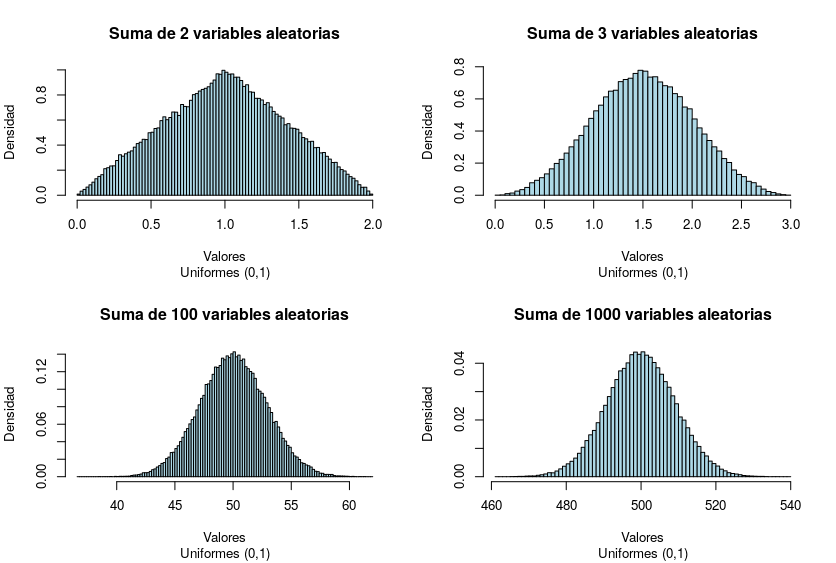
\includegraphics[height=.5\linewidth]{uniforme.png}
  \captionof{figure}{Convergencia en distribuci\'on de la suma de 2,3,100 y 1000 variables aleatorias uniformes continuas en (0,1)}
  \label{fig1}
\end{figure}

\subsubsection{Exponencial con rate=1}
En la figura \ref{fig2} puede observarse que la suma de 2 variables aleatorias con rate=1 es una distribuci\'on exponencial, y al ir agregando variables aleatorias del mismo tipo a la suma la distribuci\'on tiende a converger a una distribuci\'on normal con media y varianza cada vez mayor. Sin embargo, el proceso de normalizaci\'on procede mucho m\'as lentamente que en el caso anterior.

\begin{figure}[htpb]
\centering
  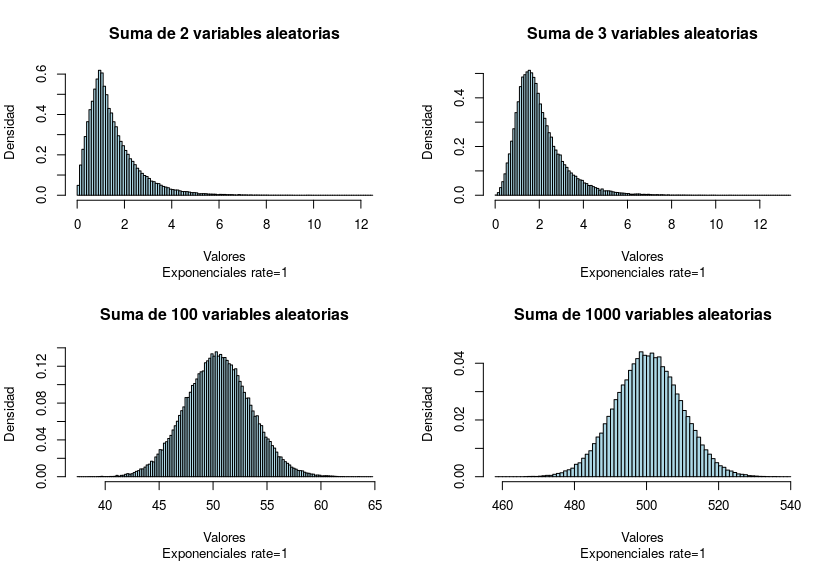
\includegraphics[height=.5\linewidth]{exponenciales.png}
  \captionof{figure}{Convergencia en distribuci\'on de la suma de 2,3,100 y 1000 variables aleatorias exponenciales con rate=1}
  \label{fig2}
\end{figure}

\subsubsection{Gaussianas estandar N(0,1)}
En la figura \ref{fig3} puede observarse que la suma de 2 variables aleatorias Gaussianas estandar toman la forma de una distribuci\'on Gaussiana N(0, $2^2$), y al ir agregando variables aleatorias del mismo tipo a la suma la distribuci\'on tiende a converger a una distribuci\'on Gaussiana N(0, $n^2$), con $n$ el n\'umero de variables aleatorias sumadas. 

\begin{figure}[htpb]
\centering
  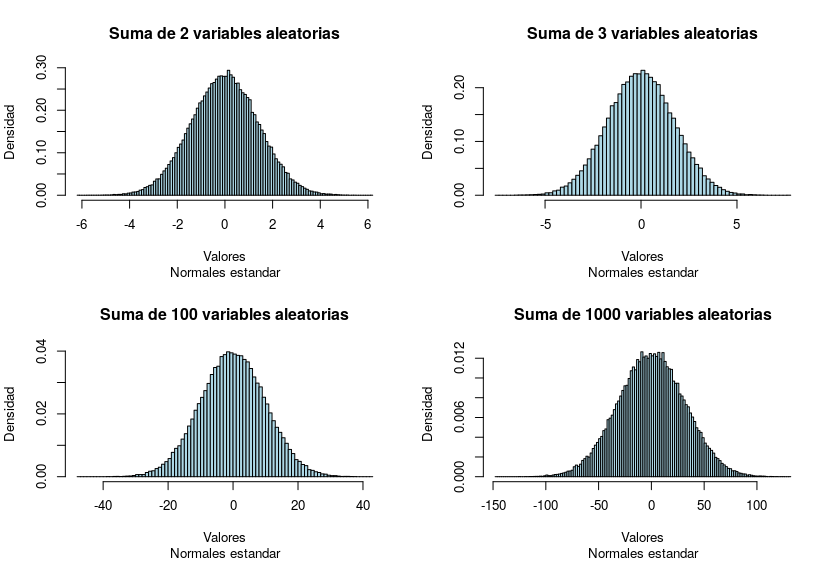
\includegraphics[height=.5\linewidth]{normales.png}
  \captionof{figure}{Convergencia en distribuci\'on de la suma de 2,3,100 y 1000 variables aleatorias Gaussianas estandar N(0,1)}
  \label{fig3}
\end{figure}

\subsubsection{Cauchy-Lorentz con $\gamma=1$ y localizaci\'on=0}
Una curiosidad de esta funci\'on de distribuci'on es que no tiene sus momentos definidos por lo que la Ley d\'ebil de los grandes n\'umeros no se cumple y por tanto el Teorema del L\'imite Central no aplica para este tipo de distribuciones. Particularmente a este tipo de distribuciones se les conoce como estables y tienen la particularidad de que una combinaci\'on lineal de variables aleatorias que siguen estas distribuciones es la misma distribuci\'on que la del primer sumando. En la figura \ref{fig4} puede observarse este fen\'omeno.



\begin{figure}[htpb]
\centering
  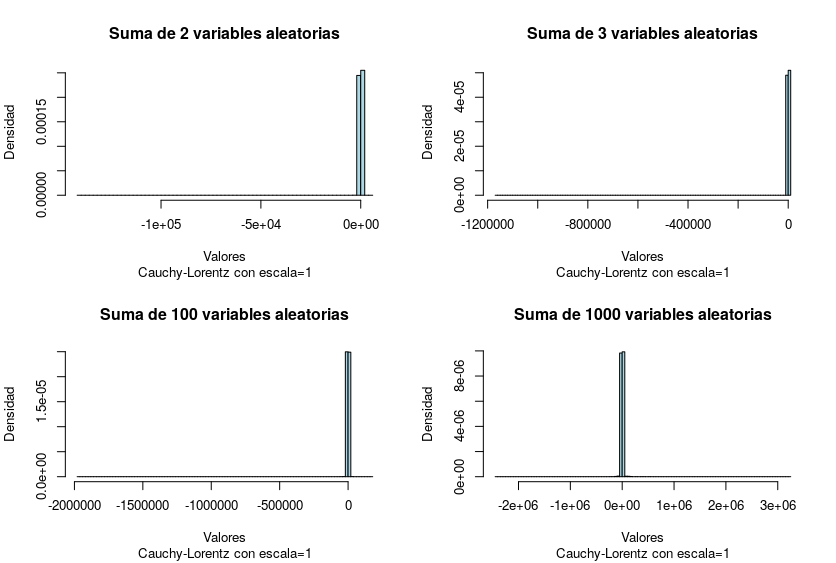
\includegraphics[height=.5\linewidth]{cauchy.png}
  \captionof{figure}{Convergencia en distribuci\'on de la suma de 2,3,100 y 1000 variables aleatorias de Cauchy-Lorentz con $\gamma=1$ y localizaci\'on=0}
  \label{fig4}
\end{figure}

\newpage
\newpage

\section{Anexo: c\'odigo}
\begin{lstlisting}{language=R}
#Limpiamos la memoria
rm(list = ls())

#Generando las distribuciones para variables 
#aleatorias uniformes continuas en (0,1)
A1 = runif(100000,0,1)
par(mfrow=c(2,2))
for (i in 1:999){
  A1 = A1+runif(100000,0,1)
  if (i==1 | i==2 | i==99| i==999) {
    texto=paste0("Suma de ", i+1, " variables aleatorias")
    hist(A1, freq=FALSE, breaks=100,main=texto, col="lightblue", sub="Uniformes (0,1)", ylab="Densidad",xlab="Valores")
    }
}


#Generando las distribuciones para variables 
#aleatorias exponenciales con lambda=1
B1 = rexp(100000, rate = 1)
par(mfrow=c(2,2))
for (i in 1:999){
  B1 = B1+runif(100000,0,1)
  if (i==1 | i==2 | i==99| i==999) {
    texto=paste0("Suma de ", i+1, " variables aleatorias")
    hist(B1, freq=FALSE, breaks=100,main=texto, col="lightblue", sub="Exponenciales rate=1", ylab="Densidad",xlab="Valores")
  }
}

#Generando las distribuciones para variables 
#aleatorias normales estandar
C1 = rnorm(100000)
par(mfrow=c(2,2))
for (i in 1:999){
  C1 = C1+rnorm(100000)
  if (i==1 | i==2 | i==99| i==999) {
    texto=paste0("Suma de ", i+1, " variables aleatorias")
    hist(C1, freq=FALSE, breaks=100,main=texto, col="lightblue", sub="Normales estandar", ylab="Densidad",xlab="Valores")
  }
}

#Generando las distribuciones para variables 
#aleatorias Cauchy-Lorentz con localizacion=0 y escala 1
D1 = rcauchy(10000,location=0, scale=1)
par(mfrow=c(2,2))
for (i in 1:9999){
  D1 = D1+rcauchy(10000,location=0, scale=1)
  if (i==1 | i==2 | i==99| i==999) {
    texto=paste0("Suma de ", i+1, " variables aleatorias")
    #plot(density(D1))
    hist(D1, freq=FALSE, breaks=100,main=texto, col="lightblue", sub="Cauchy-Lorentz con escala=1", ylab="Densidad",xlab="Valores")
  }
}


\end{lstlisting}
\end{document}